% !TeX root = RJwrapper.tex
\title{ctrialsgov: Query Data from U.S. National Library of Medicine's Clinical Trials Database}
\author{by Taylor Arnold, Michael J. Kane, Auston Wei}

\maketitle

\abstract{
Tools to create and query database from the U.S. National Library
of Medicine's Clinical Trials database <https://clinicaltrials.gov/>. Functions
provide access a variety of techniques for searching the data using range
queries, categorical filtering, and by searching for full-text keywords.
Minimal graphical tools are also provided for interactively exploring the
constructed data.
}

\section{Introduction}


\section{Creating Local Data}

Before querying the ClinicalTrials.gov data, we need to load a pre-processed
version of the data into R. There are three ways to do this. If you have
installed a copy of the data set locally into PostGRES, the data can be
created from scratch with the following block of code (it will take a couple
of minutes to finish):

\begin{example}
> library(DBI)
> library(RPostgreSQL)

> drv <- dbDriver('PostgreSQL')
> con <- DBI::dbConnect(drv, dbname="aact")
> ctgov_create_data(con)
\end{example}

Alternatively, we can download a static version of the data from GitHub and
load this into R without needing the setup a local version of the database.
This will be cached locally so that it can be re-loaded without downloading
each time. To download and load this data, use the following:

\begin{example}
> ctgov_load_cache()
\end{example}

Finally, we can load a small sample dataset (2\% of the total) that is included
with the package itself using the following:

\begin{example}
> ctgov_load_sample()
\end{example}

This is the version of the data that is used in most of the tests, examples,
and in this vignette.

\section{Running Data Queries}

The primary function for querying the dataset is called \code{ctgov\_query}. It can
be called after using any of the functions in the previous section. Here
are a few examples of how the function works. We will see a few examples here;
see the help pages for a complete list of options.

There are a number of fields in the data that use exact matches of categories.
Here, for example, we find the interventional studies:

\begin{example}
> ctgov_query(study_type = "Interventional")
# A tibble: 2,403 × 32
   nct_id      start_date phase           enrollment brief_title  official_title
   <chr>       <date>     <chr>                <int> <chr>        <chr>
 1 NCT04999163 2021-12-31 N/A                     50 Aortix Ther… Aortix Therap…
 2 NCT05002153 2021-11-30 N/A                    300 The Role of… The Role of M…
 3 NCT04472702 2021-11-30 N/A                     45 Fluoroscopi… Fluoroscopic …
 4 NCT05032157 2021-11-30 Phase 3                450 A Phase 3 S… A Multicenter…
 5 NCT04471142 2021-11-08 N/A                    270 Effectivene… Effectiveness…
 6 NCT04772651 2021-11-01 N/A                    108 Mediterrane… Mediterranean…
 7 NCT04390451 2021-11-01 Phase 1                 54 Initial Tes… Initial Testi…
 8 NCT04696861 2021-11-01 N/A                     60 Telehealth … Telehealth to…
 9 NCT03954431 2021-10-31 Phase 1/Phase 2        100 High-Resolu… Study of High…
10 NCT04273022 2021-10-31 N/A                     20 Effect of E… The Effect of…
# … with 2,393 more rows, and 26 more variables:
#   primary_completion_date <date>, study_type <chr>, rec_status <chr>,
#   completion_date <date>, last_update <date>, description <chr>,
#   eudract_num <chr>, other_id <chr>, allocation <chr>,
#   intervention_model <chr>, observational_model <chr>, primary_purpose <chr>,
#   time_perspective <chr>, masking_description <chr>,
#   intervention_model_description <chr>, sampling_method <chr>, …
\end{example}

Or, all of the interventional studies that have a primary industry sponsor:

\begin{example}
> ctgov_query(study_type = "Interventional", sponsor_type = "Industry")
# A tibble: 640 × 32
   nct_id      start_date phase           enrollment brief_title  official_title
   <chr>       <date>     <chr>                <int> <chr>        <chr>
 1 NCT04999163 2021-12-31 N/A                     50 Aortix Ther… Aortix Therap…
 2 NCT05032157 2021-11-30 Phase 3                450 A Phase 3 S… A Multicenter…
 3 NCT05029856 2021-10-04 Phase 1/Phase 2        240 Evaluation … A Randomized,…
 4 NCT04963179 2021-09-30 N/A                    154 PREvention … PREvention of…
 5 NCT04875975 2021-09-30 Phase 2                 68 A Study to … A Randomized,…
 6 NCT04909879 2021-09-30 Phase 2                100 Study of Al… Treatment of …
 7 NCT04925674 2021-09-29 Phase 1                 60 Study of HE… Phase Ic Clin…
 8 NCT04935177 2021-09-17 Phase 3                 64 Renal Funct… An Open-label…
 9 NCT04956744 2021-08-31 Phase 1                 30 A Study to … A Phase 1, Do…
10 NCT04920253 2021-08-31 N/A                    180 Real World … Real World Ev…
# … with 630 more rows, and 26 more variables: primary_completion_date <date>,
#   study_type <chr>, rec_status <chr>, completion_date <date>,
#   last_update <date>, description <chr>, eudract_num <chr>, other_id <chr>,
#   allocation <chr>, intervention_model <chr>, observational_model <chr>,
#   primary_purpose <chr>, time_perspective <chr>, masking_description <chr>,
#   intervention_model_description <chr>, sampling_method <chr>, gender <chr>,
#   minimum_age <dbl>, maximum_age <dbl>, population <chr>, criteria <chr>, …
\end{example}

A few fields have continuous values that can be searched by giving a vector
with two values. The results return any values that fall between the lower
bound (first value) and the upper bound (second value). Here, we find the
studies that have between 40 and 42 patients enrolled in them:

\begin{example}
> ctgov_query(enrollment_range = c(40, 42))
# A tibble: 125 × 32
   nct_id      start_date phase           enrollment brief_title  official_title
   <chr>       <date>     <chr>                <int> <chr>        <chr>
 1 NCT04188119 2021-09-30 Phase 2                 42 A Proof of … A Proof of Co…
 2 NCT04992975 2021-08-31 NA                      40 Brain Iron … Brain Iron To…
 3 NCT05001854 2021-08-31 Phase 2/Phase 3         40 Hemodynamic… Evaluation of…
 4 NCT04749355 2021-08-14 Phase 2                 40 Phase 2, Op… A Phase 2, Op…
 5 NCT04648319 2021-04-15 Phase 2                 40 A Study of … A Pilot Study…
 6 NCT04744779 2021-03-31 N/A                     40 Office Base… Effectiveness…
 7 NCT04841174 2021-03-30 N/A                     40 The Effect … The Effect of…
 8 NCT04808180 2021-03-25 N/A                     40 Clinical Ef… Effects of Bi…
 9 NCT04746105 2021-02-24 Phase 1                 40 A Clinical … A Study to Ev…
10 NCT04355780 2021-01-08 NA                      40 Immunologic… Immunologic F…
# … with 115 more rows, and 26 more variables: primary_completion_date <date>,
#   study_type <chr>, rec_status <chr>, completion_date <date>,
#   last_update <date>, description <chr>, eudract_num <chr>, other_id <chr>,
#   allocation <chr>, intervention_model <chr>, observational_model <chr>,
#   primary_purpose <chr>, time_perspective <chr>, masking_description <chr>,
#   intervention_model_description <chr>, sampling_method <chr>, gender <chr>,
#   minimum_age <dbl>, maximum_age <dbl>, population <chr>, criteria <chr>, …
\end{example}

Setting one end of the range to missing avoids searching for that end of the
range. For example, the following finds any studies with 1000 or more patients.

\begin{example}
> ctgov_query(enrollment_range = c(1000, NA))
# A tibble: 204 × 32
   nct_id      start_date phase   enrollment brief_title      official_title
   <chr>       <date>     <chr>        <int> <chr>            <chr>
 1 NCT05033782 2021-12-01 NA            1500 Impact of the M… Impact of the Mod…
 2 NCT05033548 2021-10-10 NA            4000 Technology Enab… Technology Enable…
 3 NCT04982614 2021-10-01 Phase 4       1400 HPV Vaccination… A Multi-site, Ope…
 4 NCT05033678 2021-08-16 NA            8000 Implementation … Teledermoscopy an…
 5 NCT04917185 2021-06-30 N/A           1000 EA for PAAS: A … Electro-acupunctu…
 6 NCT04839757 2021-06-03 NA            1400 Dengue Vaccine … Preparing for the…
 7 NCT04889924 2021-06-01 N/A           1666 ALND vs RDT in … Axillary Lymph No…
 8 NCT04472845 2021-03-30 N/A           1018 HYPofractionate… HYPofractionated …
 9 NCT04735744 2021-02-15 NA            1315 Evaluation of A… Evaluation of All…
10 NCT04626973 2021-01-15 N/A           3048 Effects of Ezet… Effects of Ezetim…
# … with 194 more rows, and 26 more variables: primary_completion_date <date>,
#   study_type <chr>, rec_status <chr>, completion_date <date>,
#   last_update <date>, description <chr>, eudract_num <chr>, other_id <chr>,
#   allocation <chr>, intervention_model <chr>, observational_model <chr>,
#   primary_purpose <chr>, time_perspective <chr>, masking_description <chr>,
#   intervention_model_description <chr>, sampling_method <chr>, gender <chr>,
#   minimum_age <dbl>, maximum_age <dbl>, population <chr>, criteria <chr>, …
\end{example}

Similarly, we can give a range of dates. These are given in the form of strings
as "YYYY-MM-DD":

\begin{example}
> ctgov_query(date_range = c("2020-01-01", "2020-02-01"))
# A tibble: 34 × 32
   nct_id      start_date phase           enrollment brief_title  official_title
   <chr>       <date>     <chr>                <int> <chr>        <chr>
 1 NCT04224597 2020-02-01 NA                      48 Evaluation … Evaluation of…
 2 NCT04255524 2020-02-01 N/A                    200 Choroidal C… OCTA to Quant…
 3 NCT04336605 2020-02-01 NA                   25000 Killing Pai… Killing Pain …
 4 NCT04218669 2020-02-01 N/A                    105 The Approac… A Clinical Ra…
 5 NCT04409613 2020-02-01 N/A                     59 Cost-Effect… Cost-Effectiv…
 6 NCT04424576 2020-01-31 NA                      60 Ovarian Mor… Trajectory of…
 7 NCT04115397 2020-01-31 Phase 4                 80 Bisphosphon… Towards Effic…
 8 NCT04497064 2020-01-30 NA                     585 Breakfast K… Breakfast Kno…
 9 NCT03892785 2020-01-27 Phase 3                200 MEthotrexat… MEthotrexate …
10 NCT03710122 2020-01-23 Phase 2/Phase 3        102 Vancomycin … A Prospective…
# … with 24 more rows, and 26 more variables: primary_completion_date <date>,
#   study_type <chr>, rec_status <chr>, completion_date <date>,
#   last_update <date>, description <chr>, eudract_num <chr>, other_id <chr>,
#   allocation <chr>, intervention_model <chr>, observational_model <chr>,
#   primary_purpose <chr>, time_perspective <chr>, masking_description <chr>,
#   intervention_model_description <chr>, sampling_method <chr>, gender <chr>,
#   minimum_age <dbl>, maximum_age <dbl>, population <chr>, criteria <chr>, …
\end{example}

Finally, we can also search free text fields using keywords. The following for
example finds and study that includes the phrase "lung cancer" (ignoring
case) in the description field:

\begin{example}
> ctgov_query(description_kw = "lung cancer")
# A tibble: 59 × 32
   nct_id      start_date phase   enrollment brief_title      official_title
   <chr>       <date>     <chr>        <int> <chr>            <chr>
 1 NCT04814056 2021-06-01 Phase 4         15 To Evaluate the… An Open-Labeled, …
 2 NCT04629027 2021-03-03 NA              80 Evaluation Syst… Establishment of …
 3 NCT04179305 2020-10-25 N/A             58 Giving Informat… Giving Informatio…
 4 NCT04452877 2020-08-19 Phase 2         20 A Study of Dabr… An Open-Label, Si…
 5 NCT04422392 2020-07-13 Phase 2        107 Neoadjuvant PD-… Neoadjuvant PD-1 …
 6 NCT04120454 2020-03-16 Phase 2         34 Ramucirumab and… An Investigator-S…
 7 NCT04332367 2019-12-19 Phase 2         59 Carboplatin, Ta… Phase II, Single-…
 8 NCT04309955 2019-12-01 N/A             60 Modified Versus… Randomized Clinic…
 9 NCT04151940 2019-09-26 NA              40 PET/CT Changes … An Observational …
10 NCT04081688 2019-08-21 Phase 1         15 Atezolizumab an… A Phase I Trial o…
# … with 49 more rows, and 26 more variables: primary_completion_date <date>,
#   study_type <chr>, rec_status <chr>, completion_date <date>,
#   last_update <date>, description <chr>, eudract_num <chr>, other_id <chr>,
#   allocation <chr>, intervention_model <chr>, observational_model <chr>,
#   primary_purpose <chr>, time_perspective <chr>, masking_description <chr>,
#   intervention_model_description <chr>, sampling_method <chr>, gender <chr>,
#   minimum_age <dbl>, maximum_age <dbl>, population <chr>, criteria <chr>, …
\end{example}

We can search two terms at once as well, by default it finds things that match
at least one of the terms:

\begin{example}
> ctgov_query(description_kw = c("lung cancer", "colon cancer"))
# A tibble: 59 × 32
   nct_id      start_date phase   enrollment brief_title      official_title
   <chr>       <date>     <chr>        <int> <chr>            <chr>
 1 NCT04814056 2021-06-01 Phase 4         15 To Evaluate the… An Open-Labeled, …
 2 NCT04629027 2021-03-03 NA              80 Evaluation Syst… Establishment of …
 3 NCT04179305 2020-10-25 N/A             58 Giving Informat… Giving Informatio…
 4 NCT04452877 2020-08-19 Phase 2         20 A Study of Dabr… An Open-Label, Si…
 5 NCT04422392 2020-07-13 Phase 2        107 Neoadjuvant PD-… Neoadjuvant PD-1 …
 6 NCT04120454 2020-03-16 Phase 2         34 Ramucirumab and… An Investigator-S…
 7 NCT04332367 2019-12-19 Phase 2         59 Carboplatin, Ta… Phase II, Single-…
 8 NCT04309955 2019-12-01 N/A             60 Modified Versus… Randomized Clinic…
 9 NCT04151940 2019-09-26 NA              40 PET/CT Changes … An Observational …
10 NCT04081688 2019-08-21 Phase 1         15 Atezolizumab an… A Phase I Trial o…
# … with 49 more rows, and 26 more variables: primary_completion_date <date>,
#   study_type <chr>, rec_status <chr>, completion_date <date>,
#   last_update <date>, description <chr>, eudract_num <chr>, other_id <chr>,
#   allocation <chr>, intervention_model <chr>, observational_model <chr>,
#   primary_purpose <chr>, time_perspective <chr>, masking_description <chr>,
#   intervention_model_description <chr>, sampling_method <chr>, gender <chr>,
#   minimum_age <dbl>, maximum_age <dbl>, population <chr>, criteria <chr>, …
\end{example}

But the `match\_all` flag can be set to search for both terms at the same time
(here, that returns no matches):

\begin{example}
> ctgov_query(description_kw = c("lung cancer", "colon cancer"), match_all = TRUE)
# A tibble: 0 × 32
# … with 32 variables: nct_id <chr>, start_date <date>, phase <chr>,
#   enrollment <int>, brief_title <chr>, official_title <chr>,
#   primary_completion_date <date>, study_type <chr>, rec_status <chr>,
#   completion_date <date>, last_update <date>, description <chr>,
#   eudract_num <chr>, other_id <chr>, allocation <chr>,
#   intervention_model <chr>, observational_model <chr>, primary_purpose <chr>,
#   time_perspective <chr>, masking_description <chr>, …
\end{example}

Other keyword fields include \code{official\_title\_kw},
\code{source\_kw} and \code{criteria\_kw}.

Any of the options can be combined as needed.

\begin{example}
> ctgov_query(
+   description_kw = "cancer",
+   enrollment_range = c(100, 200),
+   date_range = c("2019-01-01", "2020-02-01")
+ )
# A tibble: 5 × 32
  nct_id start_date phase enrollment brief_title official_title primary_complet…
  <chr>  <date>     <chr>      <int> <chr>       <chr>          <date>
1 NCT04… 2020-01-22 N/A          120 Symptom Ma… Improving Sym… 2025-10-01
2 NCT04… 2020-01-07 Phas…        121 Study Eval… A Phase 2, Op… 2023-07-31
3 NCT04… 2020-01-01 NA           100 Extraordin… Extraordinary… 2022-01-01
4 NCT03… 2019-03-12 NA           115 Moderately… Moderately Hy… 2022-05-31
5 NCT03… 2019-02-20 N/A          160 The Effect… The Effect of… 2019-05-31
# … with 25 more variables: study_type <chr>, rec_status <chr>,
#   completion_date <date>, last_update <date>, description <chr>,
#   eudract_num <chr>, other_id <chr>, allocation <chr>,
#   intervention_model <chr>, observational_model <chr>, primary_purpose <chr>,
#   time_perspective <chr>, masking_description <chr>,
#   intervention_model_description <chr>, sampling_method <chr>, gender <chr>,
#   minimum_age <dbl>, maximum_age <dbl>, population <chr>, criteria <chr>, …
\end{example}

Finally, we can also pass a current version of the data set to the query
function, rather than starting with the full data set. This is useful when
you want to combine queries in a more complex way. For example, this is
equivalent to the above:

\begin{example}
> library(dplyr)

> ctgov_query() %>%
+   ctgov_query(description_kw = "cancer") %>%
+   ctgov_query(enrollment_range = c(100, 200)) %>%
+   ctgov_query(date_range = c("2019-01-01", "2020-02-01"))
# A tibble: 5 × 32
  nct_id start_date phase enrollment brief_title official_title primary_complet…
  <chr>  <date>     <chr>      <int> <chr>       <chr>          <date>
1 NCT04… 2020-01-22 N/A          120 Symptom Ma… Improving Sym… 2025-10-01
2 NCT04… 2020-01-07 Phas…        121 Study Eval… A Phase 2, Op… 2023-07-31
3 NCT04… 2020-01-01 NA           100 Extraordin… Extraordinary… 2022-01-01
4 NCT03… 2019-03-12 NA           115 Moderately… Moderately Hy… 2022-05-31
5 NCT03… 2019-02-20 N/A          160 The Effect… The Effect of… 2019-05-31
# … with 25 more variables: study_type <chr>, rec_status <chr>,
#   completion_date <date>, last_update <date>, description <chr>,
#   eudract_num <chr>, other_id <chr>, allocation <chr>,
#   intervention_model <chr>, observational_model <chr>, primary_purpose <chr>,
#   time_perspective <chr>, masking_description <chr>,
#   intervention_model_description <chr>, sampling_method <chr>, gender <chr>,
#   minimum_age <dbl>, maximum_age <dbl>, population <chr>, criteria <chr>, …
\end{example}

\section{Data Visualization}

\begin{figure}[t!]
  \centering
  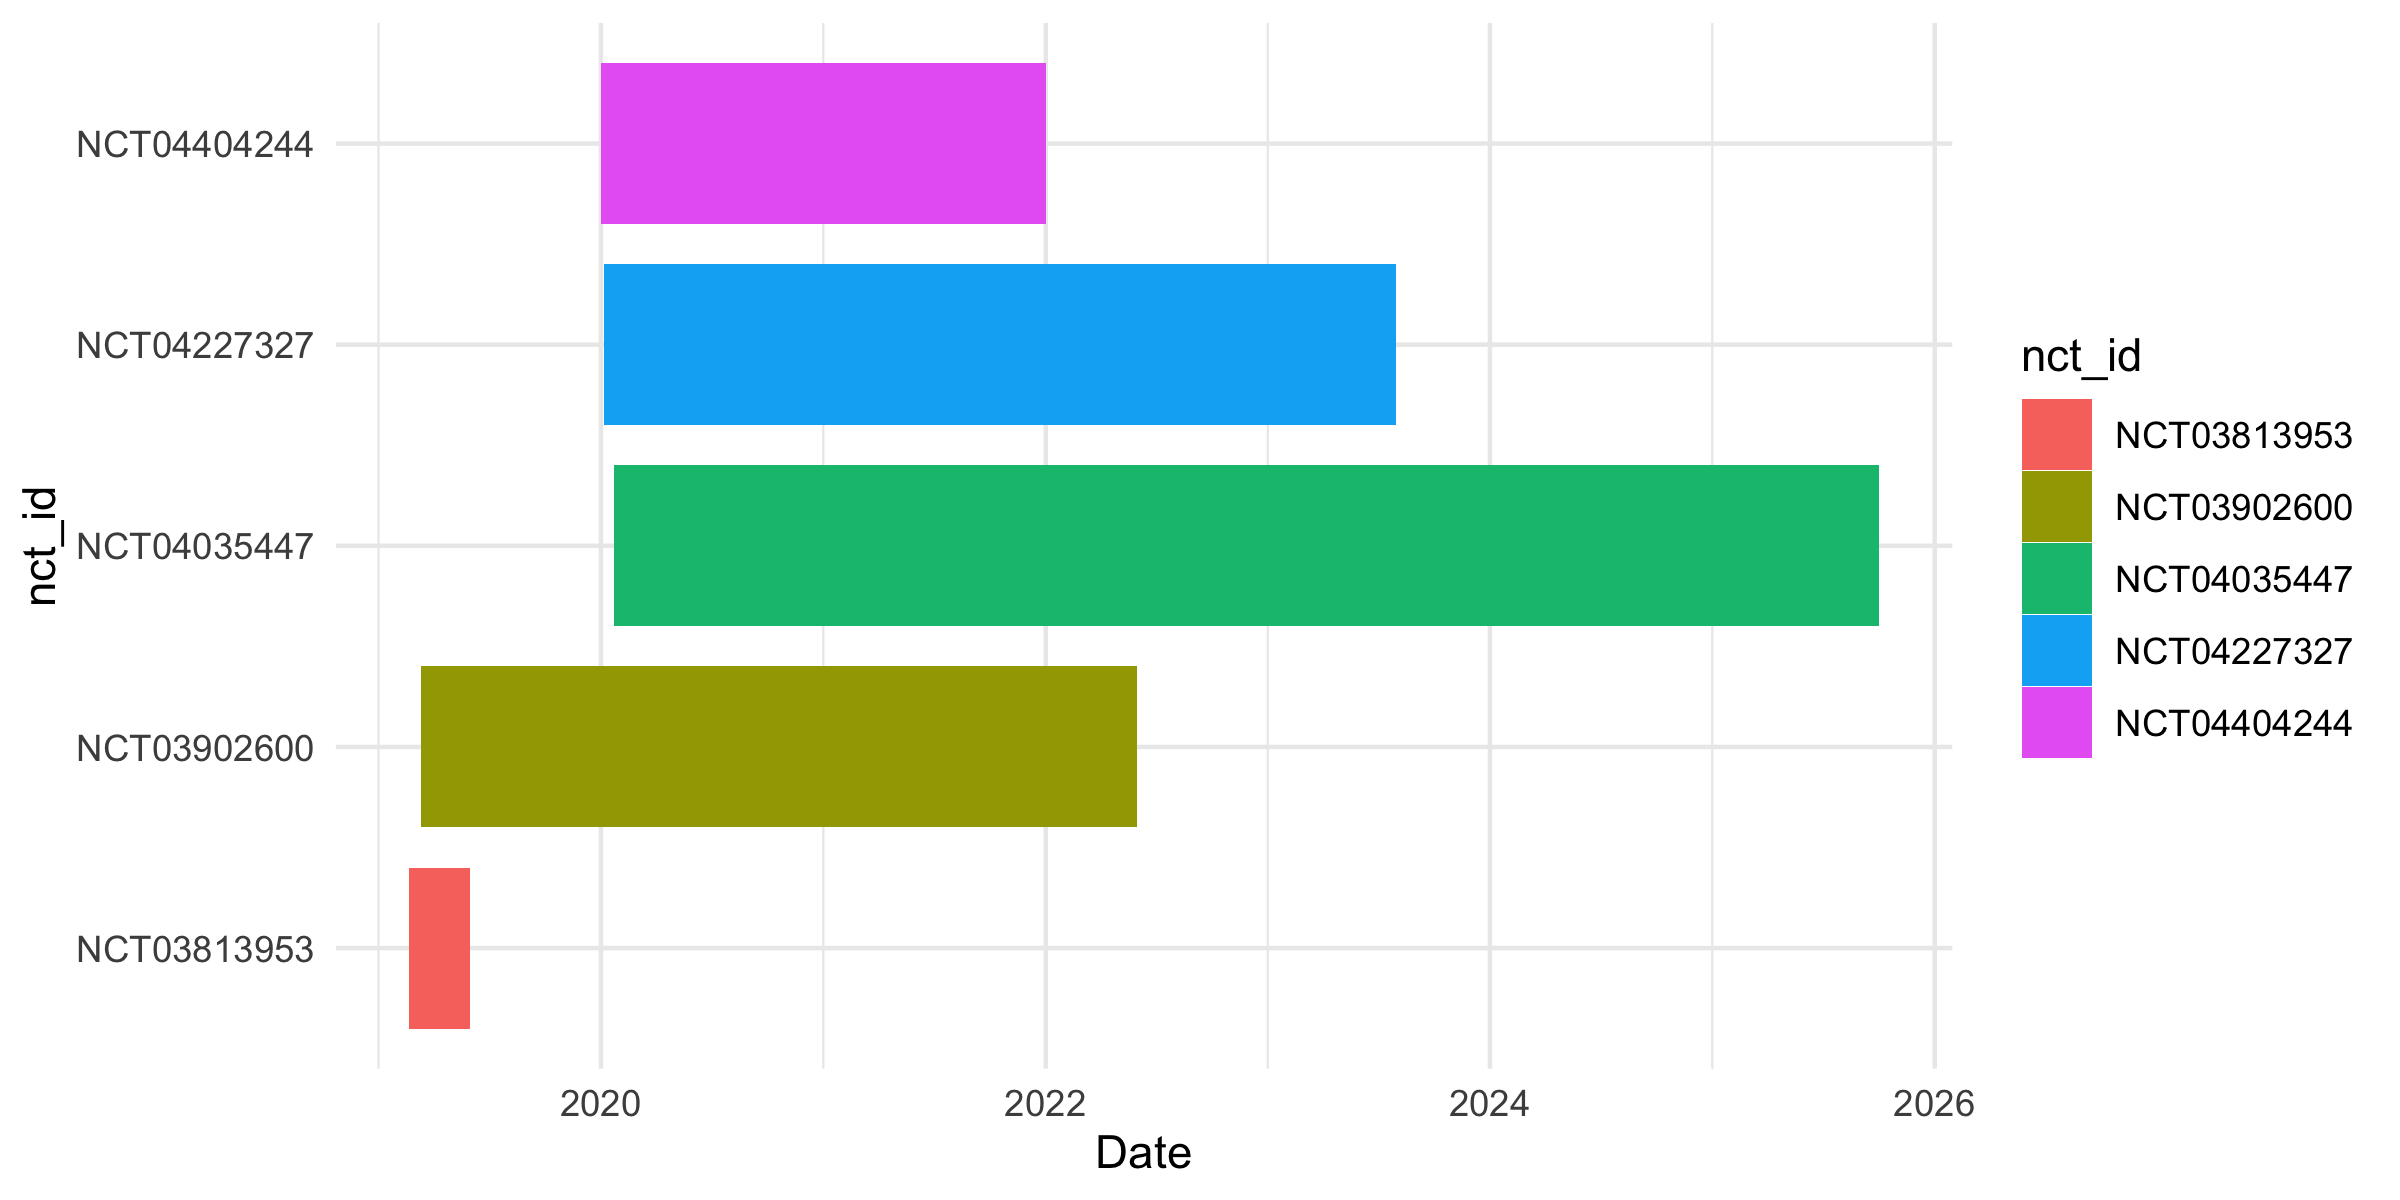
\includegraphics[width=0.95\textwidth]{fig1.png}
  \caption{Static Output from the timeline graphic interface.}
  \label{figure:timeline}
\end{figure}

The package also contains a number of tools for visualizing the output.
Here is one example:

\begin{example}
> ctgov_query(
+    description_kw = "cancer",
+    enrollment_range = c(100, 200),
+    date_range = c("2019-01-01", "2020-02-01")
+  ) %>%
+  ctgov_plot_timeline() +
+    ggplot2::theme_minimal()
\end{example}

\section{Text Analysis}

\subsection{Keywords in Context}

The function \code{ctgov\_kwic} highlights all of the occurances of a term within
its context (the few words before and after the term occurs). For example, if
we want to show the occurances of the term "bladder" in the titles of the
interventional trials we can do this:

\begin{example}
> z <- ctgov_query(study_type = "Interventional")
> ctgov_kwic("bladder", z[['brief_title']])
ible Local Advanved |Bladder| Cancer
 of Sulforaphane in |Bladder| Cancer Chemoprevent
      Comparison of |Bladder| Filling vs. Non-Fil
tment of Overactive |Bladder|/Urge Incontinence
in the Detection of |Bladder| Cancer in the Surve
A-F Betafood on Gall|bladder| and Liver Function.
Non-Muscle Invasive |Bladder| Cancer
iopathic Overactive |Bladder| With Urinary Incont
tion for Overactive |Bladder|
anced or Metastatic |Bladder| Cancer
     Autologous Neo-|Bladder| Construct in Non-Ne
urogenic Overactive |Bladder| and Urge Predominan
 AMG 706 on the Gall|bladder| in Advanced Solid T
Men With Overactive |Bladder|.
\end{example}

The function also has an option to include a title along with each occurance
that is printed alongside each row. Here we will print the NCT id for each
trial:

\begin{example}
> z <- ctgov_query(study_type = "Interventional")
> ctgov_kwic("bladder", z[['brief_title']], z[['nct_id']])
[NCT04553939] ible Local Advanved |Bladder| Cancer
[NCT03517995]  of Sulforaphane in |Bladder| Cancer Chemoprevent
[NCT04210479]       Comparison of |Bladder| Filling vs. Non-Fil
[NCT03535857] tment of Overactive |Bladder|/Urge Incontinence
[NCT02560584] in the Detection of |Bladder| Cancer in the Surve
[NCT01981343] A-F Betafood on Gall|bladder| and Liver Function.
[NCT01625260] Non-Muscle Invasive |Bladder| Cancer
[NCT00910845] iopathic Overactive |Bladder| With Urinary Incont
[NCT00912314] tion for Overactive |Bladder|
[NCT00635726] anced or Metastatic |Bladder| Cancer
[NCT00594139]      Autologous Neo-|Bladder| Construct in Non-Ne
[NCT00594139] urogenic Overactive |Bladder| and Urge Predominan
[NCT00448786]  AMG 706 on the Gall|bladder| in Advanced Solid T
[NCT00282932] Men With Overactive |Bladder|.
\end{example}

There are some other options that can be used to change the way that the
output is displayed. The default (shown above) prints the results out using
the \code{cat} function. Other options return the results as a character vector of
data frame, which are useful for further post-processing. There is also a
flag \code{use\_color} that prints the term in color rather than with pipes; it looks
great in a terminal or RStudio but does not display correctly when knit to
HTML.

\subsection{TF-IDF}

We can use a technique called term frequence-inverse document frequency (TF-IDF)
to determine the most important words in a collection of of text fields. To
implement this in R we will use the \code{ctgov\_tfidf} function:

\begin{example}
> z <- ctrialsgov::ctgov_query()
> tfidf <- ctgov_tfidf(z[['description']])
> print(tfidf, n = 30)
# A tibble: 3,074 × 2
     doc terms
   <int> <chr>
 1     0 aortix|heightened|aki|providing|abdominal
 2     1 pollution|ms|air|viral|france
 3     2 fmt|diversity|microbiota|weight|gut
 4     3 nerves|landmarks|bony|guidance|knee
 5     4 antihistamines|h1|inadequately|spontaneous|suffering
 6     5 bandage|seroma|drain|categorical|variables
 7     6 vagal|mediterranean|nerve|diet|depression
 8     7 veterans|peer|whole|steps|structured
 9     8 suicidal|ideation|telehealth|engagement|counseling
10     9 bct|ce|breast|structures|cancers
11    10 athletes|pathways|exercise|biomarkers|strenuous
12    11 acetylsalicylic|vessels|artery|affects|acid
13    12 mhealth|90|monitoring|organ|impact
14    13 cascade|sugar|glucose|sensor|doctors
15    14 variant|b1351|cov2|sars|b16172
16    15 scenario|uncertainties|oncological|relating|real
17    16 itch|epigenetic|mechanisms|chronic|antagonists
18    17 9vhpv|1526|hiv|living|uninfected
19    18 dengue|fever|permeability|five|vascular
20    19 influenza|icu|aspergillosis|eortc|pathogen
21    20 cannabigerol|cbg|thc|appetite|stimulating
22    21 antibiotics|decide|how|parent|prescribed
23    22 counseling|education|behavior|behavioral|his
24    23 intrauterine|adhesiolysis|leaf|film|named
25    24 purifiers|cardiopulmonary|indicators|students|air
26    25 donepezil|french|alzheimers|efficiency|authorities
27    26 avelumab|checkpoint|breast|immune|aspirin
28    27 dbs|ps|expectations|pd|preoperative
29    28 brentuximab|vedotin|classic|nivolumab|checkpoint
30    29 wl|calorie|aas|ba|crc
# … with 3,044 more rows
\end{example}

The default takes the lower case version of the terms, but (particularly with
acronyms) it may be better to preserve the capitalization of the terms. Here is
how we can do that in this example:

\begin{example}
> tfidf <- ctgov_tfidf(z[['description']], tolower = FALSE)
> print(tfidf, n = 30)
# A tibble: 3,074 × 2
     doc terms
   <int> <chr>
 1     0 heightened|AKI|providing|abdominal|System
 2     1 pollution|MS|air|viral|France
 3     2 FMT|diversity|microbiota|weight|gut
 4     3 nerves|landmarks|bony|guidance|knee
 5     4 H1|inadequately|spontaneous|suffering|comparison
 6     5 seroma|drain|categorical|variables|regression
 7     6 Mediterranean|vagal|nerve|diet|depression
 8     7 Whole|Veterans|package|Health|mental
 9     8 suicidal|ideation|telehealth|engagement|counseling
10     9 BCT|CE|breast|structures|cancers
11    10 athletes|pathways|exercise|biomarkers|strenuous
12    11 Acetylsalicylic|Acid|vessels|artery|affects
13    12 mHealth|90|monitoring|organ|impact
14    13 sugar|glucose|sensor|doctors|venous
15    14 variant|CoV2|SARS|Beta|vaccine
16    15 scenario|uncertainties|oncological|relating|real
17    16 itch|epigenetic|mechanisms|chronic|antagonists
18    17 9vHPV|1526|HIV|living|uninfected
19    18 dengue|fever|permeability|five|vascular
20    19 influenza|ICU|aspergillosis|EORTC|pathogen
21    20 THC|appetite|stimulating|subjective|analgesic
22    21 antibiotics|decide|how|prescribed|pneumonia
23    22 counseling|education|behavioral|his|behavior
24    23 intrauterine|adhesiolysis|film|named|adhesion
25    24 purifiers|cardiopulmonary|air|students|indicators
26    25 French|Alzheimers|efficiency|controversy|reimbursed
27    26 checkpoint|Immune|breast|immune|aspirin
28    27 DBS|PS|expectations|PD|preoperative
29    28 vedotin|brentuximab|nivolumab|classic|checkpoint
30    29 WL|calorie|AAs|BA|CRC
# … with 3,044 more rows
\end{example}

We can also refine the results by including fewer rare terms. The argument
\code{min\_df} specifies the minimal proportion of documents that must contain a term
for it to be returned as a keyword; the upper bound can also be specified
with the argument \code{max\_df}.

\begin{example}
> tfidf <- ctgov_tfidf(z[['description']], min_df = 0.02, max_df = 0.2)
> print(tfidf, n = 30)
# A tibble: 3,072 × 2
     doc terms
   <int> <chr>
 1     0 injury|support|cardiovascular|performance|feasibility
 2     1 impact|care|health|risk|better
 3     2 weight|loss|body|10|least
 4     3 but|these|compare|two|which
 5     4 adult|tolerability|chronic|placebo|participants
 6     5 outcome|multiple|analysis|evaluated|performed
 7     6 depression|function|assess|efficacy
 8     7 support|health|level|care|primary
 9     8 improved|support|high|intervention|care
10     9 breast|out|being|performed|if
11    10 exercise|events|associated|compared|inflammation
12    11 condition|heart|information|blood|when
13    12 impact|days|objective|outcome|secondary
14    13 levels|diabetes|blood|level|device
15    14 vaccine|novel|include|label|open
16    15 about|new|studies|free|benefit
17    16 chronic|examine|testing|disorder|while
18    17 vaccine|women|among|those|dose
19    18 death|treat|syndrome|pilot|evaluation
20    19 pulmonary|incidence|observational|multi|identify
21    20 alone|combination|assess|effects
22    21 how|often|children|if|not
23    22 diseases|chronic|follow|it|changes
24    23 novel|aims|controlled|randomized|efficacy
25    24 explore|aims|changes|function|health
26    25 non|disease|cognitive|approach|currently
27    26 breast|immune|approximately|called|cancer
28    27 postoperative|improvement|result|brain|specific
29    28 treated|cells|may|cancer|ability
30    29 prevention|interventions|weight|its|no
# … with 3,042 more rows
\end{example}

Any number of text fields can be passed to the \code{ctgov\_tokens} function; all of
the fields for a specific trial are pasted together and treated a single block
of text.

\subsection{Document Similarity}

Finally, the package also provides a function for producing similarity scores
based on the text fields of the studies. Here, we will produce a similarity
matrix based on the description field of Interventional, Industry-sponsored,
Phase 2 trials.

\begin{example}
> z <- ctgov_query(
+    study_type = "Interventional", sponsor_type = "Industry", phase = "Phase 2"
+  )
+  scores <- ctgov_text_similarity(z[['description']], min_df = 0, max_df = 0.1)
+  dim(scores)
[1] 147 147
\end{example}

The returned value is a square matrix with one row and one colum for each
clinical trial in the set. We can use these scores to find studies that are
particularly close to one another in the words used within their descriptions.
Here for example we can see five studies that use similar terms in their
descriptions:

\begin{example}
> index <- order(scores[,100], decreasing = TRUE)[1:5]
> z[['brief_title']][index]
[1] "AL-38583 Ophthalmic Solution for Allergic Conjunctivitis Associated Inflammation"
[2] "Safety and Efficacy of BRM421 for Dry Eye Syndrome"
[3] "Phosphorylcholine PC-mAb Effects in Subjects With Elevated Lipoprotein a"
[4] "Safety, Clinical Tolerability and Immunogenicity of Increasing Doses of gpASIT+TM"
[5] "Phase 2 Clinical Trial of CartiLife in the United States"
\end{example}

Further post-processing can be done with the similarity scores, such as spectral
clustering and dimensionality reduction.

\section{Case Study}


\section{Conclusions}


\bibliography{RJreferences}

\address{Taylor Arnold\\
  University of Richmond\\
  410 Westhampton Way, Richmond, VA 23173\\
  U.S.A.\\
  (0000-0003-0576-0669)\\
  \email{tarnold2@richmond.edu}}

\address{Auston Wei\\
  Cleveland Clinic\\
  9500 Euclid Avenue, Cleveland, Ohio 44195\\
  U.S.A.\\
  \email{auston@telperian.com}}

\address{Michael Kane\\
  Yale University\\
  New Haven, CT 06520\\
  U.S.A.\\
  ( 0000-0003-1899-6662)\\
  \email{michael.kane@yale.edu}}
